\section{Introducing Garage}

%%%%%%%%%%%%%%%%%%%%%%%%%%%%%%%%%%%%%%%%%%%%%%%%%%%%%%%%%%%%%%%%%%%
\begin{frame}{Brought to you by the Deuxfleurs association}

\begin{block}{\textbf{deuxfleurs.fr} -- a libre hosting association with a vision}
``Shifting the current structure of the Internet from a world of a few very large service providers, to a world where services are hosted by a variety of smaller organisations.''	
\end{block}


\begin{block}{Our goals}
\begin{itemize}
	\item To propose performant \& reliable libre services for the masses
	\item To host and administer our infrastructure ourselves
	\item To allow members to contribute storage/compute nodes
	\item Resilience: for availability \& the sysadmins' sleep 
	\item Conceptual simplicity to ease onboarding \& demistify hosting
\end{itemize}
\end{block}


\end{frame}

%%%%%%%%%%%%%%%%%%%%%%%%%%%%%%%%%%%%%%%%%%%%%%%%%%%%%%%%%%%%%%%%%%%
\begin{frame}{The lacking state of the practice}

\begin{block}{Object storage fitted our needs}
\begin{itemize}
	\item Distributed by design
	\item Objects are replicated
	\item Conceptually simple
\end{itemize}
\end{block}
\vfill 

\begin{block}{Existing object stores did not}
	\begin{itemize}
		\item Too specific / complex 
		\item Resource hungry 
		\item Hidden constraints 
	\end{itemize}
\end{block}
\vfill

We developed Garage, an object store with minimal functionality.

It works, and serves our static sites and media.

\end{frame}

%%%%%%%%%%%%%%%%%%%%%%%%%%%%%%%%%%%%%%%%%%%%%%%%%%%%%%%%%%%%%%%%%%%
\begin{frame}{Introducing Garage}

\centering
\url{garagehq.deuxfleurs.fr}

\url{git.deuxfleurs.fr/Deuxfleurs/garage}


\includegraphics[width=.4\columnwidth]{figures/garage_distributed.png}
\vfill

\raggedright
\begin{itemize}
	\item Distributed data store
	\item Based on DynamoDB object store (P2P!)
	\item Modular data types/protocols with CRDTs:
	\begin{itemize}
		\item Done: objects (media, static sites, backups...) via S3 API 
		\item To do: e-mails via IMAP protocol, and more
	\end{itemize}
\end{itemize}

\end{frame}

%%%%%%%%%%%%%%%%%%%%%%%%%%%%%%%%%%%%%%%%%%%%%%%%%%%%%%%%%%%%%%%%%%%
\begin{frame}[t]{The \textbf{RING}}

\centering
\fullcite{decandia_dynamo:_2007}
\vspace{3ex}

\only<1>{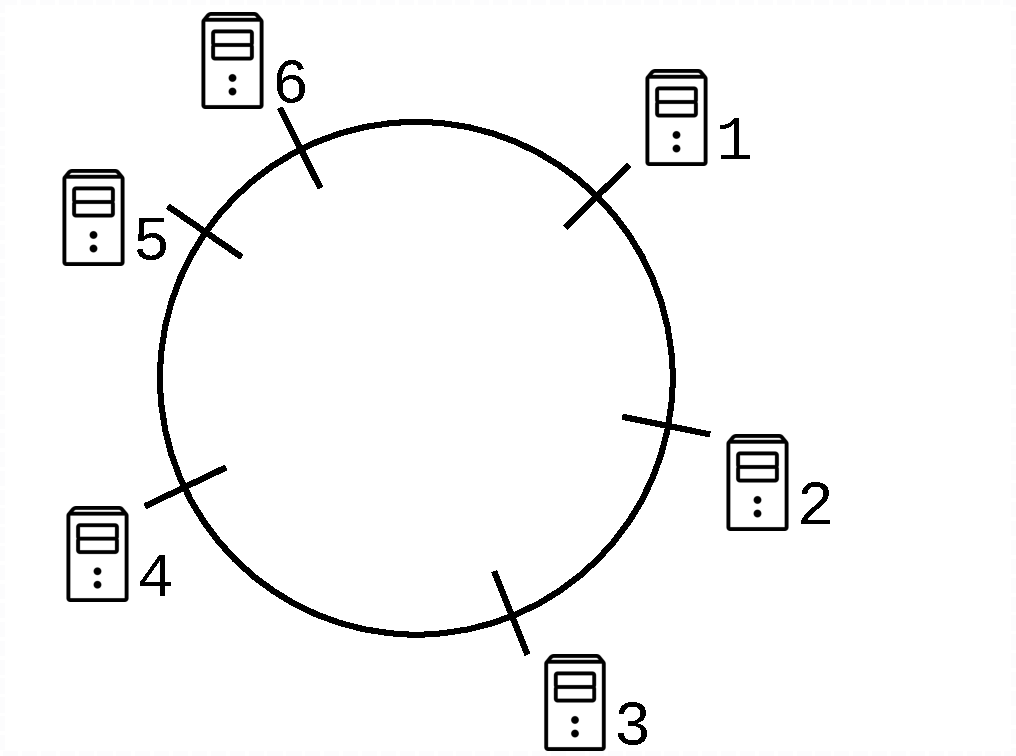
\includegraphics[width=.5\columnwidth]{figures/c1.pdf}}%
\only<2>{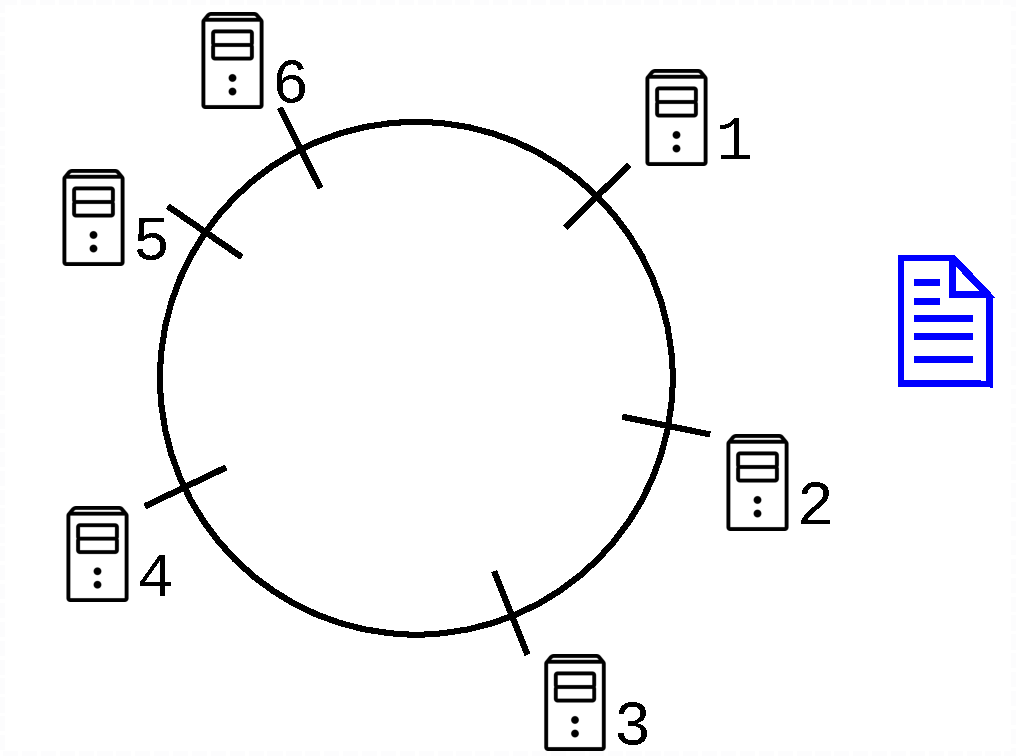
\includegraphics[width=.5\columnwidth]{figures/c2.pdf}}%
\only<3>{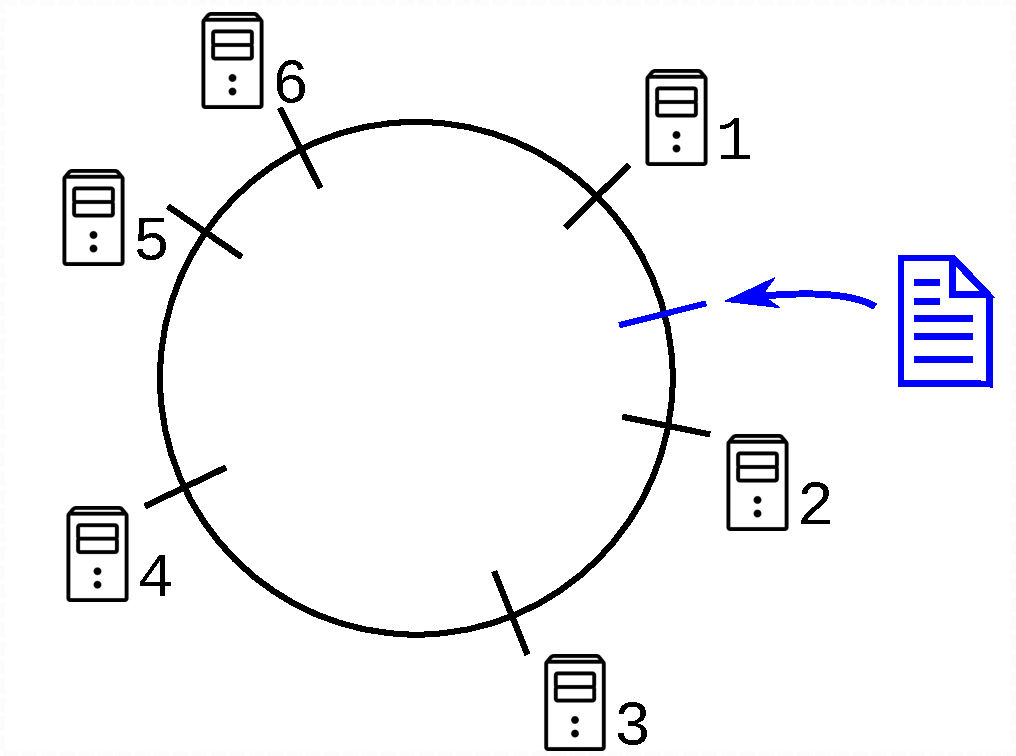
\includegraphics[width=.5\columnwidth]{figures/c3.pdf}}%
\only<4>{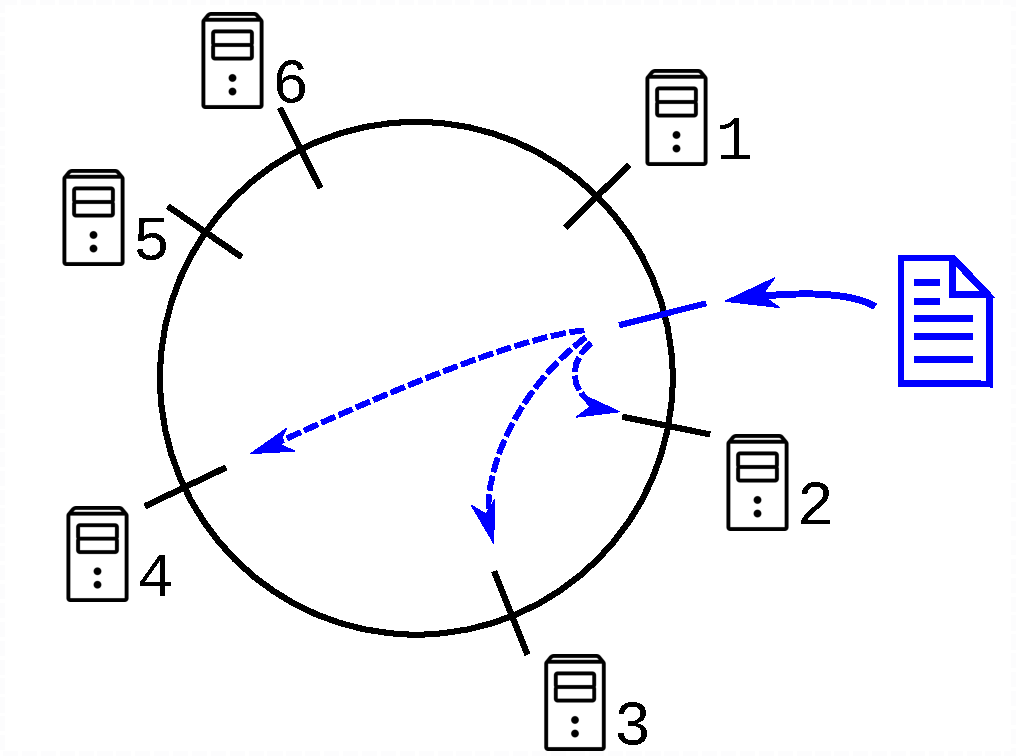
\includegraphics[width=.5\columnwidth]{figures/c4.pdf}}%
\vspace{5ex}

%\raggedright
\only<1>{Each node is assigned a unique ID on the circular address space.}%
\only<2-3>{When a new object is added to the store...}%
\only<3>{\\ It is assigned a unique ID (its \emph{key}) on the address space.}%
\only<4>{The $R$ nodes after the object are in charge of replicating it.}%

\end{frame}


%%%%%%%%%%%%%%%%%%%%%%%%%%%%%%%%%%%%%%%%%%%%%%%%%%%%%%%%%%%%%%%%%%%
\begin{frame}{Distributed metadata}

\centering
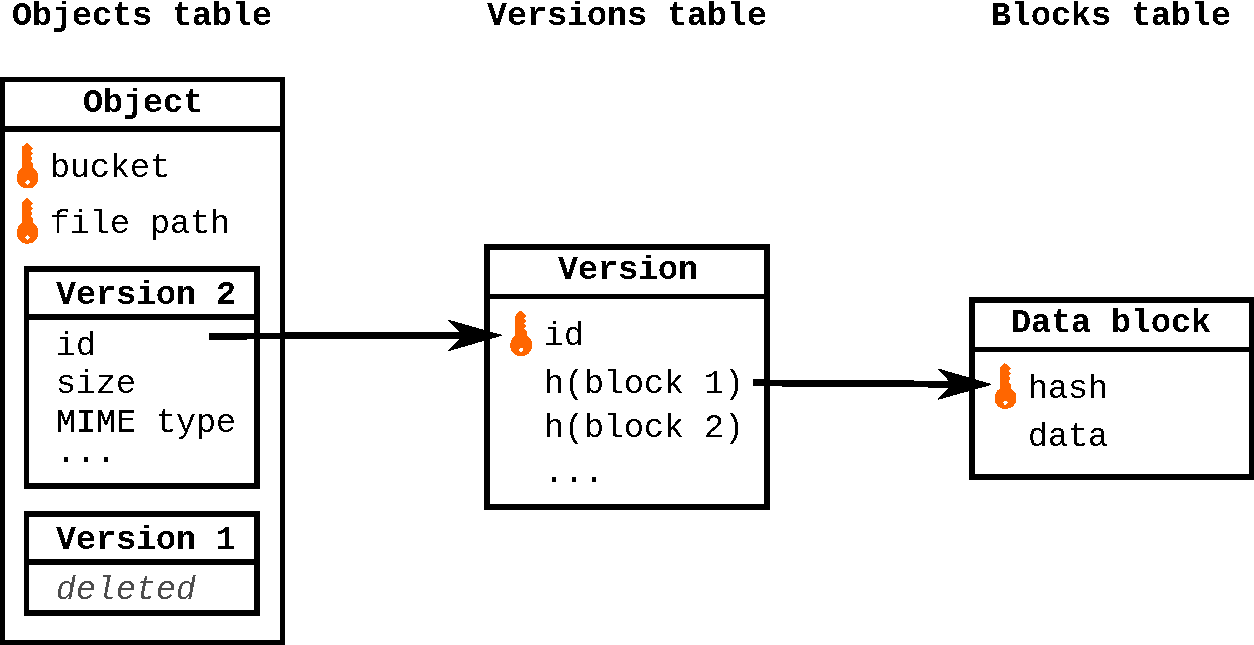
\includegraphics[width=.8\columnwidth]{figures/garage_tables.pdf}
\vfill

The objects, versions and blocks are all stored in the ring.

\end{frame}


%%%%%%%%%%%%%%%%%%%%%%%%%%%%%%%%%%%%%%%%%%%%%%%%%%%%%%%%%%%%%%%%%%%
\begin{frame}{Written in Rust}

\begin{columns}
\column{.65\columnwidth}
Entirely written in Rust!
\column{.35\columnwidth}
\centering

\includegraphics[width=.85\columnwidth]{figures/rustacean-flat-happy.png}
\end{columns}
\vfill

\begin{columns}
\column[t]{.6\columnwidth}
	\textbf{Pros:}
	\begin{itemize}
		\item Compiled and fast
		\item Features prevent usual mistakes:

		strongly typed, immutable by default, ownership instead of GC...

		\item Best of several paradigms:

		imperative, OO, functional

		\item Good libraries for network programmings:

		serialization, http, async/await...
	\end{itemize}
\column[t]{.4\columnwidth}
	\textbf{Cons}:
	\begin{itemize}
		\item Steep learning curve
		\item Long compilation times
		\item Compiler rage
	\end{itemize}
\end{columns}

\end{frame}